\section{Softwares and Tools Used}

\subsection{KiCad}
KiCad has been extensively used to design the \gls{pcb} for the circuit. We have used KiCad with the following specificaiton.
\begin{itemize}
\item[~]Version: (25-Oct-2014 BZR 4029)-stable
\item[~]Build: wxWidgets 3.0.2 (debug,wchar\_t,compiler with C++ ABI 1002,GCC 4.9.2,wx containers,compatible with 2.8)
\item[~]Platform: Linux 3.19.0-22-generic x86\_64, 64 bit, Little endian, wxGTK
Boost version: 1.53.0
\end{itemize}

\subsection{Proteus}
Proteus is a simulation software for various designs. It is a handy tool to test programs and embedded electronics designs. It can be used to simulate programs for microcontroller as well as  test various circuits before implementing them into hardware. We have used Proteas 7.8 for the most part.

\subsection{Programmer}
Avrdude has been used as a tool to communicate between program written in computer and the microcontroller on which the program is to be written. The programmer is made form ATMEGA8 microcontroller. We opted to get one already available in the market.
\begin{figure}[h]
	\centering
	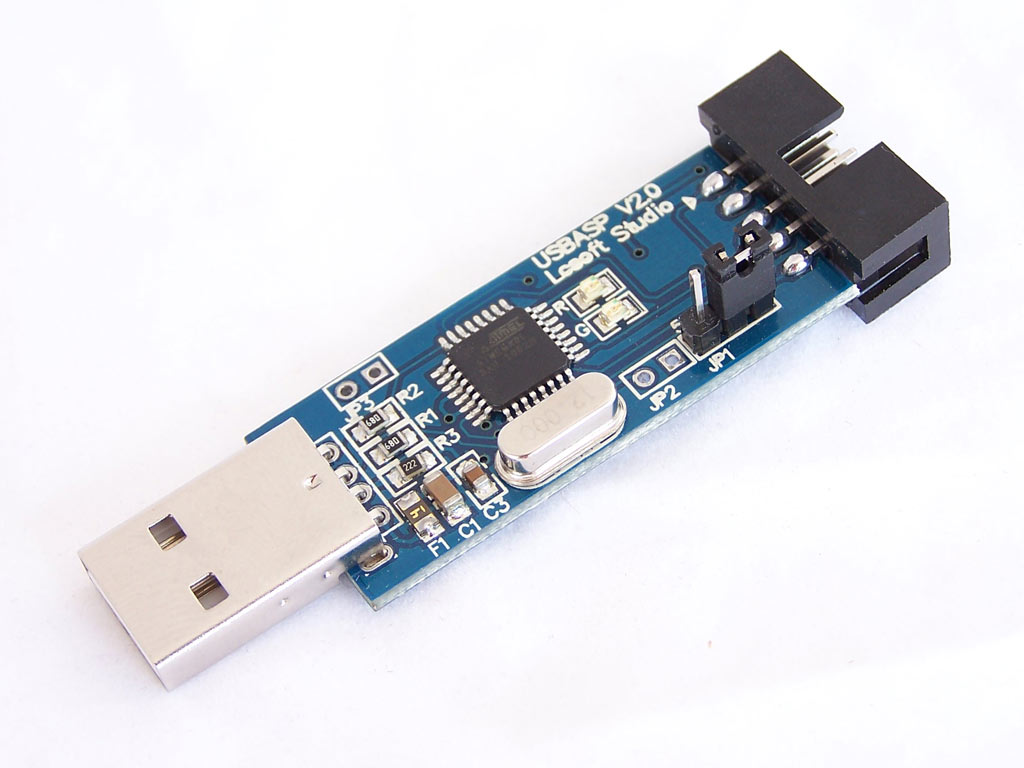
\includegraphics[scale=0.18]{Images/Programmer.jpg}
	\caption{USBasp Programmer}
	\label{fig:Programmer}
\end{figure}


\subsection{AVR GCC compiler}
AVR-GCC is a compiler that takes C language high level code and creates a binary source which can be uploaded into an AVR micro controller. Once code in 'C' is written for a particular project, AVR-GCC will turn C code into assembly language files. 

Individual assembler files are then converted into object files. Object files are files of code that AVR chips could run. The linker AVR-ld will take all these assembler files, and cross-reference functions names to create one single object file. The linker will also take modules from the 'C' library and make them into a single object. Normally this linked object is in ELF format and furthermore AVR-objcopy is used to generate a HEX format file.

